% questions.tex —— 2006 年·普通高等学校招生考试·江苏卷 · 题目内容片段（无答案）
% 由 tools/generate_projects.py 依来源总账自 2006/2006_数学真题_江苏_试题.md 生成，勿手改（改源 MD 后重跑）


\begin{gktip}
\textbf{来源及状态}：据本机固定 PDF 第 1–2 页逐题目视转录；文件 SHA-256 与给定 source manifest 记录一致。首页可见题签为“2006 普通高等学校招生考试（江苏卷）”。题签和字节指纹只能确认本次读取的固定副本及其页内文字，不能认证发布者、版次、来源链或官方原件身份。PDF 未见答案、解析或评分页；题签未标科类，本稿不推定文理科或其他变体。

\textbf{源页定位}：PDF 第 1 页（印刷页码 302）含 Q1–Q18；第 2 页（印刷页码 303）含 Q19–Q21。选择题 Q1–Q10，填空题 Q11–Q16，解答题 Q17–Q21。源页未标各题分值或总分。

\textbf{题图位置}：Q9（两个正四棱锥与正方体）、Q10（信号源及五个接收器的线路）、Q18（正六棱柱与正六棱锥帐篷）、Q19（折叠前后两幅图）均有矢量图稿，按固定候选 PDF 相应页可辨的结构、标签与虚实线重绘；仅呈现固定副本可见信息，不据答案补画图上不可见部分，也不表示比例尺寸。固定 PDF 的发布者、版次、来源链及官方身份仍未核实。
\end{gktip}

\gkpart{一、选择题}

\begin{question}
\gkti{1}已知 $a\in\mathbb R$，函数 $f(x)=\sin x-|a|$，$x\in\mathbb R$ 为奇函数，则 $a=$\mbox{（　　）}

（A）$0$　（B）$1$　（C）$-1$　（D）$\pm1$

\end{question}
\begin{question}
\gkti{2}圆 $(x-1)^2+(y+\sqrt3)^2=1$ 的切线方程中有一个是\mbox{（　　）}

（A）$x-y=0$　（B）$x+y=0$　（C）$x=0$　（D）$y=0$

\end{question}
\begin{question}
\gkti{3}某人 5 次上班途中所花的时间（单位：分钟）分别为 $x,y,10,11,9$。已知这组数据的平均数为 $10$，方差为 $2$，则 $|x-y|$ 的值为\mbox{（　　）}

（A）$1$　（B）$2$　（C）$3$　（D）$4$

\end{question}
\begin{question}
\gkti{4}为了得到函数 $y=2\sin\left(\dfrac{x}{3}+\dfrac{\pi}{6}\right)$，$x\in\mathbb R$ 的图象，只需把函数 $y=2\sin x$，$x\in\mathbb R$ 的图象上所有的点\mbox{（　　）}

（A）向左平移 $\dfrac{\pi}{6}$ 个单位长度，再把所得各点的横坐标缩短到原来的 $\dfrac13$ 倍（纵坐标不变）

（B）向右平移 $\dfrac{\pi}{6}$ 个单位长度，再把所得各点的横坐标缩短到原来的 $\dfrac13$ 倍（纵坐标不变）

（C）向左平移 $\dfrac{\pi}{6}$ 个单位长度，再把所得各点的横坐标伸长到原来的 $3$ 倍（纵坐标不变）

（D）向右平移 $\dfrac{\pi}{6}$ 个单位长度，再把所得各点的横坐标伸长到原来的 $3$ 倍（纵坐标不变）

\end{question}
\begin{question}
\gkti{5}$\left(\sqrt{x}-\dfrac{1}{3x}\right)^{10}$ 的展开式中含 $x$ 的正整数指数幂的项数是\mbox{（　　）}

（A）$0$　（B）$2$　（C）$4$　（D）$6$

\end{question}
\begin{question}
\gkti{6}已知两点 $M(-2,0),N(2,0)$，点 $P$ 为坐标平面内的动点，满足
\nopagebreak[4]
\[\left|\overrightarrow{MN}\right|\cdot\left|\overrightarrow{MP}\right|+\overrightarrow{MN}\cdot\overrightarrow{NP}=0,\]
则动点 $P(x,y)$ 的轨迹方程为\mbox{（　　）}

（A）$y^2=8x$　（B）$y^2=-8x$　（C）$y^2=4x$　（D）$y^2=-4x$

\end{question}
\begin{question}
\gkti{7}若 $A\text{、}B\text{、}C$ 为三个集合，$A\cup B=B\cap C$，则一定有\mbox{（　　）}

（A）$A\subseteq C$　（B）$C\subseteq A$　（C）$A\ne C$　（D）$A\ne\varnothing$

\end{question}
\begin{question}
\gkti{8}设 $a\text{、}b\text{、}c$ 是互不相等的正数，则下列不等式中不恒成立的是\mbox{（　　）}

（A）$|a-b|\leqslant|a-c|+|b-c|$

（B）$a^2+\dfrac{1}{a^2}\geqslant a+\dfrac{1}{a}$

（C）$|a-b|+\dfrac{1}{a-b}\geqslant2$

（D）$\sqrt{a+3}-\sqrt{a+1}\leqslant\sqrt{a+2}-\sqrt a$

\Needspace{0.4\textheight}
\end{question}
\begin{question}
\gkti{9}两个相同的正四棱锥组成如图所示的几何体，可放入棱长为 $1$ 的正方体内，使正四棱锥的底面 $ABCD$ 与正方体的某一个平面平行，且各顶点均在正方体的面上，则这样的几何体体积的可能值有\mbox{（　　）}

（A）$1$ 个　（B）$2$ 个　（C）$3$ 个　（D）无穷多个
\nopagebreak[4]
\begin{center}% Source-relative PDF page 1, Q9 (printed page 302).
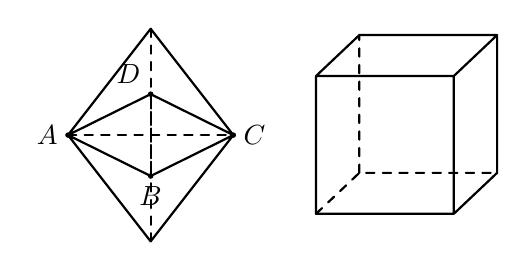
\begin{tikzpicture}[line cap=round,line join=round,thick]
  % Two congruent square pyramids sharing the square ABCD.
  \coordinate (A) at (0,1.0); \coordinate (B) at (1.05,0.48);
  \coordinate (C) at (2.1,1.0); \coordinate (D) at (1.05,1.52);
  \coordinate (T) at (1.05,2.35); \coordinate (S) at (1.05,-0.35);
  \draw[dashed] (A)--(C) (T)--(B) (S)--(D);
  \draw (A)--(D)--(C) (A)--(B)--(C) (T)--(A) (T)--(C) (S)--(A) (S)--(C);
  \fill (A) circle (1pt) node[left] {$A$};
  \fill (B) circle (1pt) node[below] {$B$};
  \fill (C) circle (1pt) node[right] {$C$};
  \fill (D) circle (1pt) node[above left] {$D$};
  % Unit cube; hidden rear-left edges are dashed.
  \begin{scope}[xshift=3.15cm]
    \coordinate (a) at (0,0); \coordinate (b) at (1.75,0);
    \coordinate (c) at (1.75,1.75); \coordinate (d) at (0,1.75);
    \coordinate (e) at (0.55,0.52); \coordinate (f) at (2.3,0.52);
    \coordinate (g) at (2.3,2.27); \coordinate (h) at (0.55,2.27);
    \draw (a)--(b)--(c)--(d)--cycle (b)--(f)--(g)--(c) (d)--(h)--(g);
    \draw[dashed] (a)--(e)--(f) (e)--(h);
  \end{scope}
\end{tikzpicture}
\end{center}
\nopagebreak[4]
\Needspace{0.4\textheight}
\end{question}
\begin{question}
\gkti{10}图中有一个信号源和五个接收器。接收器与信号源在同一个串联线路中时，就能接收到信号，否则就不能接收到信号。若将图中左端的六个接线点随机地平均分成三组，将右端的六个接线点也随机地平均分成三组，再把所有六组中每组的两个接线点用导线连接，则这五个接收器能同时接收到信号的概率是\mbox{（　　）}

（A）$\dfrac{4}{45}$　（B）$\dfrac{1}{36}$　（C）$\dfrac{4}{15}$　（D）$\dfrac{8}{15}$
\nopagebreak[4]
\begin{center}% Source-relative PDF page 1, Q10 (printed page 302).
\begin{tikzpicture}[line cap=round,line join=round,thick]
  \foreach \y in {0,-0.62,-1.24,-1.86,-2.48,-3.10} {
    \draw (0,\y)--(4.4,\y);
    \fill (0,\y) circle (1.15pt);
    \fill (4.4,\y) circle (1.15pt);
  }
  \draw (2.2,0) circle (0.24);
  \draw (2.2,0) circle (0.085);
  \node[above=5pt] at (2.2,0.24) {信号源};
  \foreach \y in {-0.62,-1.24,-1.86,-2.48,-3.10}
    \draw (1.82,\y-0.15) rectangle (2.58,\y+0.15);
\end{tikzpicture}
\end{center}
\nopagebreak[4]
\end{question}
\gkpart{二、填空题}

\begin{question}
\gkti{11}在 $\triangle ABC$ 中，已知 $BC=12$，$A=60^\circ$，$B=45^\circ$，则 $AC=$ \gkblank{}。

\end{question}
\begin{question}
\gkti{12}设变量 $x,y$ 满足约束条件
\nopagebreak[4]
\[\begin{cases}2x-y\leqslant2,\\x-y\geqslant-1,\\x+y\geqslant1,\end{cases}\]
则 $z=2x+3y$ 的最大值为 \gkblank{}。

\end{question}
\begin{question}
\gkti{13}今有 2 个红球，3 个黄球，4 个白球，同色球不加以区分，将这 9 个球排成一列有 \gkblank{} 种不同的方法。（用数字作答）

\end{question}
\begin{question}
\gkti{14}$\cot20^\circ\cos10^\circ+\sqrt3\sin10^\circ\tan70^\circ-2\cos40^\circ=$ \gkblank{}。

\end{question}
\begin{question}
\gkti{15}对正整数 $n$，设曲线 $y=x^n(1-x)$ 在 $x=2$ 处的切线与 $y$ 轴交点的纵坐标为 $a_n$，则数列 $\left\{\dfrac{a_n}{n+1}\right\}$ 的前 $n$ 项和的公式是 \gkblank{}。

\end{question}
\begin{question}
\gkti{16}不等式 $\log_2\left(x+\dfrac1x+6\right)\leqslant3$ 的解集为 \gkblank{}。

\end{question}
\begingroup
\renewcommand{\gkpart}[1]{\Needspace{0.4\textheight}\subsection*{#1}\nopagebreak}
\gkpart{三、解答题}
\endgroup

\begin{question}
\gkti{17}已知三点 $P(5,2)\text{、}F_1(-6,0)\text{、}F_2(6,0)$。

（1） 求以 $F_1\text{、}F_2$ 为焦点且过点 $P$ 的椭圆的标准方程；

（2） 设点 $P\text{、}F_1\text{、}F_2$ 关于直线 $y=x$ 的对称点分别为 $P'\text{、}F_1'\text{、}F_2'$，求以 $F_1'\text{、}F_2'$ 为焦点且过点 $P'$ 的双曲线的标准方程。

\Needspace{0.4\textheight}
\end{question}
\begin{question}
\gkti{18}请您设计一个帐篷。它下部的形状是高为 $1\text{ m}$ 的正六棱柱，上部的形状是侧棱长为 $3\text{ m}$ 的正六棱锥（如图所示）。试问当帐篷的顶点 $O$ 到底面中心 $O_1$ 的距离为多少时，帐篷的体积最大？
\nopagebreak[4]
\begin{center}% Source-relative PDF page 1, Q18 (printed page 302).
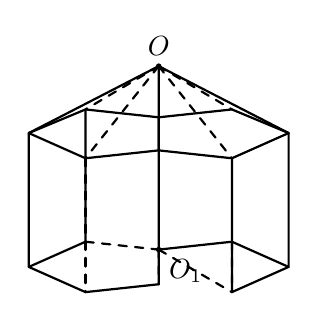
\begin{tikzpicture}[line cap=round,line join=round,thick]
  % Upper hexagonal pyramid, joined to a hexagonal prism below.
  \coordinate (O) at (1.65,3.65);
  \coordinate (A) at (0,2.8); \coordinate (B) at (0.72,3.1);
  \coordinate (C) at (1.65,3.0); \coordinate (D) at (2.58,3.1);
  \coordinate (E) at (3.3,2.8); \coordinate (F) at (2.58,2.48);
  \coordinate (G) at (1.65,2.58); \coordinate (H) at (0.72,2.48);
  \coordinate (I) at (0,1.1); \coordinate (J) at (0.72,1.42);
  \coordinate (K) at (1.65,1.32); \coordinate (L) at (2.58,1.42);
  \coordinate (M) at (3.3,1.1); \coordinate (N) at (2.58,0.78);
  \coordinate (Q) at (1.65,0.88); \coordinate (R) at (0.72,0.78);
  \draw (A)--(B)--(C)--(D)--(E) (E)--(F)--(G)--(H)--(A);
  \draw (O)--(A) (O)--(C) (O)--(E) (O)--(G);
  \draw[dashed] (O)--(B) (O)--(D) (O)--(F) (O)--(H);
  \draw (A)--(I)--(J)--(B) (C)--(K)--(G) (E)--(M)--(N)--(F);
  \draw (I)--(R)--(Q)--(K)--(L)--(M);
  \draw[dashed] (J)--(K) (J)--(R) (K)--(Q) (K)--(N) (L)--(N);
  \draw[dashed] (H)--(R) (G)--(Q) (F)--(N);
  \fill (O) circle (1pt) node[above] {$O$};
  \fill (K) circle (1pt) node[below right] {$O_1$};
\end{tikzpicture}
\end{center}
\nopagebreak[4]
\Needspace{0.4\textheight}
\end{question}
\begin{question}
\gkti{19}在正三角形 $ABC$ 中，$E\text{、}F\text{、}P$ 分别是 $AB\text{、}AC\text{、}BC$ 边上的点，满足 $AE:EB=CF:FA=CP:PB=1:2$（如图 1）。将 $\triangle AEF$ 沿 $EF$ 折起到 $\triangle A_1EF$ 的位置，使二面角 $A_1-EF-B$ 成直二面角，连接 $A_1B\text{、}A_1P$（如图 2）。

（1） 求证：$A_1E\perp$ 平面 $BEP$；

（2） 求直线 $A_1E$ 与平面 $A_1BP$ 所成角的大小；

（3） 求二面角 $B-A_1P-F$ 的大小。（用反三角函数表示）
\nopagebreak[4]
\begin{center}% Source-relative PDF page 2, Q19 (printed page 303); left=图1, right=图2.
\begin{tikzpicture}[line cap=round,line join=round,thick]
  % 图1: equilateral triangle ABC, with E,F,P on the indicated sides.
  \begin{scope}
    \coordinate (A) at (1.25,2.45); \coordinate (B) at (0,0); \coordinate (C) at (2.5,0);
    \coordinate (E) at (0.42,0.82); \coordinate (F) at (1.67,0.82);
    \coordinate (P) at (1.67,0);
    \draw (A)--(B)--(C)--cycle (E)--(F) (P)--(F);
    \foreach \p/\pos in {A/above,B/below left,C/below right,E/left,F/above right,P/below}
      \fill (\p) circle (0.9pt) node[\pos] {$\p$};
    \node[below=5pt] at (1.25,-0.3) {图 1};
  \end{scope}
  \node at (3.15,1.15) {$\Longrightarrow$};
  % 图2: folded solid; hidden edges and the EF hinge continuation are dashed.
  \begin{scope}[xshift=3.8cm]
    \coordinate (B) at (0,0); \coordinate (P) at (1.5,0.48); \coordinate (C) at (2.6,0);
    \coordinate (E) at (1.02,0.87); \coordinate (F) at (2.03,0.92);
    \coordinate (A1) at (1.48,2.3);
    \draw (B)--(P)--(C) (B)--(A1)--(C) (A1)--(F)--(C) (A1)--(P) (A1)--(E) (E)--(B) (E)--(F) (F)--(P);
    \draw[dashed] (B)--(F) (E)--(P);
    \foreach \p/\pos in {A1/above,B/below left,C/below right,E/left,F/right,P/below}
      \fill (\p) circle (0.9pt) node[\pos] {$\p$};
    \node[below=5pt] at (1.3,-0.3) {图 2};
  \end{scope}
\end{tikzpicture}
\end{center}
\nopagebreak[4]
\end{question}
\begin{question}
\gkti{20}设 $a$ 为实数，设函数 $f(x)=a\sqrt{1-x^2}+\sqrt{1+x}+\sqrt{1-x}$ 的最大值为 $g(a)$。

（1） 设 $t=\sqrt{1+x}+\sqrt{1-x}$，求 $t$ 的取值范围，并把 $f(x)$ 表示为 $t$ 的函数 $m(t)$；

（2） 求 $g(a)$；

（3） 试求满足 $g(a)=g\left(\dfrac1a\right)$ 的所有实数 $a$。

\end{question}
\begingroup
\renewenvironment{question}{\Needspace{0.05\textheight}}{}
\begin{question}
\gkti{21}设数列 $\{a_n\},\{b_n\},\{c_n\}$ 满足：$b_n=a_n-a_{n+2}$，$c_n=a_n+2a_{n+1}+3a_{n+2}$（$n=1,2,3,\cdots$）。证明：$\{a_n\}$ 为等差数列的充分必要条件是 $\{c_n\}$ 为等差数列且 $b_n\leqslant b_{n+1}$（$n=1,2,3,\cdots$）。


\end{question}
\endgroup